This section describes the interconnected component in a water distributed network (WDN) using Graph Theory. Furthermore thee component classes will be examined, ie. pipes, pumps and valves.

When using graph theory as an analytical tool the incident matrix $H$ comes in handy when describing the connection between edges and nodes. The rules shown below has been used as guidelines when writing up the incident matrix for a graph network. 

\subsubsection{The Incident Matrix}
\begin{equation*}
	H_{i,j} = \begin{cases}
		-1 & \text{If the $j^{th}$ edge enters the $i^{th}$ node} \\
		0 & \text{If the $j^{th}$ edge is not connected to the $i^{th}$ node} \\
		1 & \text{If the $j^{th}$ edge s leaving the $i^{th}$ node}
	\end{cases}
\end{equation*} %Description of the incident matrix

\subsubsection{The Loop Marix}
The loop-matrix can be calculated in one of two ways. The first one is shown in the equation below

\begin{equation} \label{Bmatrix}
	B = \begin{bmatrix}
		I & -\bar{H}_{C}^{T}\cdot\bar{H}_{T}^{-T}
	\end{bmatrix}
\end{equation}


The other method is more graphical but can be formulated as follows: JEG KAN IKKE HUSKE REGLEN.

\newpage
\subsection{Simplified system}
\begin{figure}[h!]
	\centering
	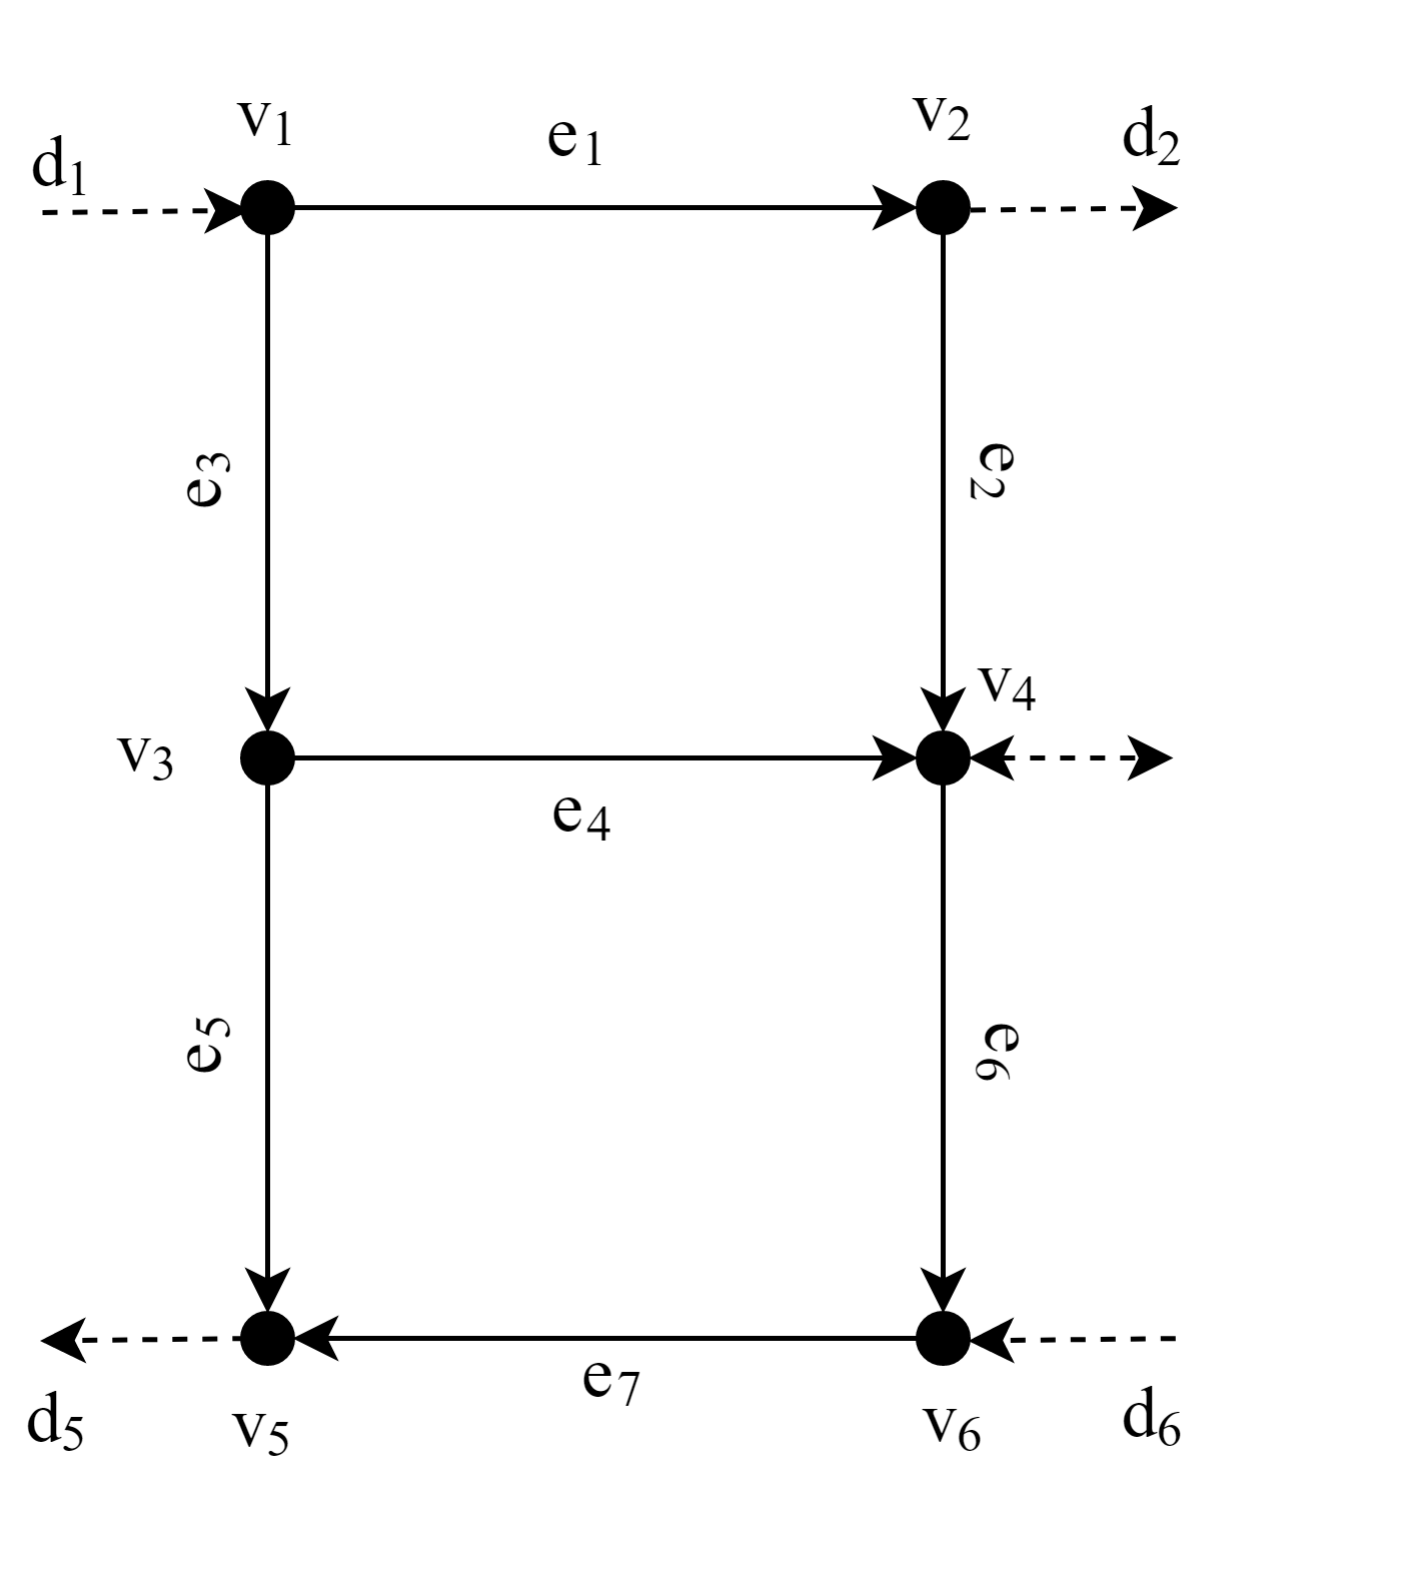
\includegraphics[width=0.5\textwidth]{Pictures/Graph.png}
	\caption{Graph of simplified WDN network \cite{Rathore930}}
	\label{fig:graph}
\end{figure}

When applying the rules shown above for the simplified graph model of the WDN the incident matrix in \cref{eq:H_simplified}.

\begin{equation}
	H = \begin{bmatrix}
		1 & 0 & 1 & 0 & 0 & 0 & 0\\
		-1 & 1 & 0 & 0 & 0 & 0 & 0\\
		0 & 0 & -1 & 1 & 1 & 0 & 0\\
		0 & -1 & 0 & -1 & 0 & 1 & 0\\
		0 & 0 & 0 & 0 & -1 &  0  & -1\\
		0 & 0 & 0 & 0 & 0 & -1 & 1
	\end{bmatrix}
	\label{eq:H_simplified}
\end{equation} %The incident matrix for system


The reduced incident matrix by taking an arbitrary vertex as a reference, and removing that vertex-row from \cref{eq:H_simplified}. We chose the $4^{th}$ vertex, which results in the following reduced incident matrix:
\begin{equation}
	\bar{H} = \begin{bmatrix}
		1 & 0 & 1 & 0 & 0 & 0 & 0\\
		-1 & 1 & 0 & 0 & 0 & 0 & 0\\
		0 & 0 & -1 & 1 & 1 & 0 & 0\\
		0 & 0 & 0 & 0 & -1 &  0  & -1\\
		0 & 0 & 0 & 0 & 0 & -1 & 1
	\end{bmatrix}
\end{equation}

Chords and edges of the spanning tree

\begin{equation*} 
	\begin{split}
		E_{C} &= \{e_{1},e_{4}\}   \\ E_{T} &= \{e_2,e_3,e_5,e_6,e_7\}
	\end{split}
\end{equation*}


\begin{equation}
	B = \begin{bmatrix}
		1 & 0 & 1 & -1 & -1 & 1 & 1\\
		0 & 1 & 0 & 0 & -1 & 1 & 1\\
	\end{bmatrix}
\end{equation}
\newpage

\subsection{Detailed system}

\begin{figure}[h]
	\centering
	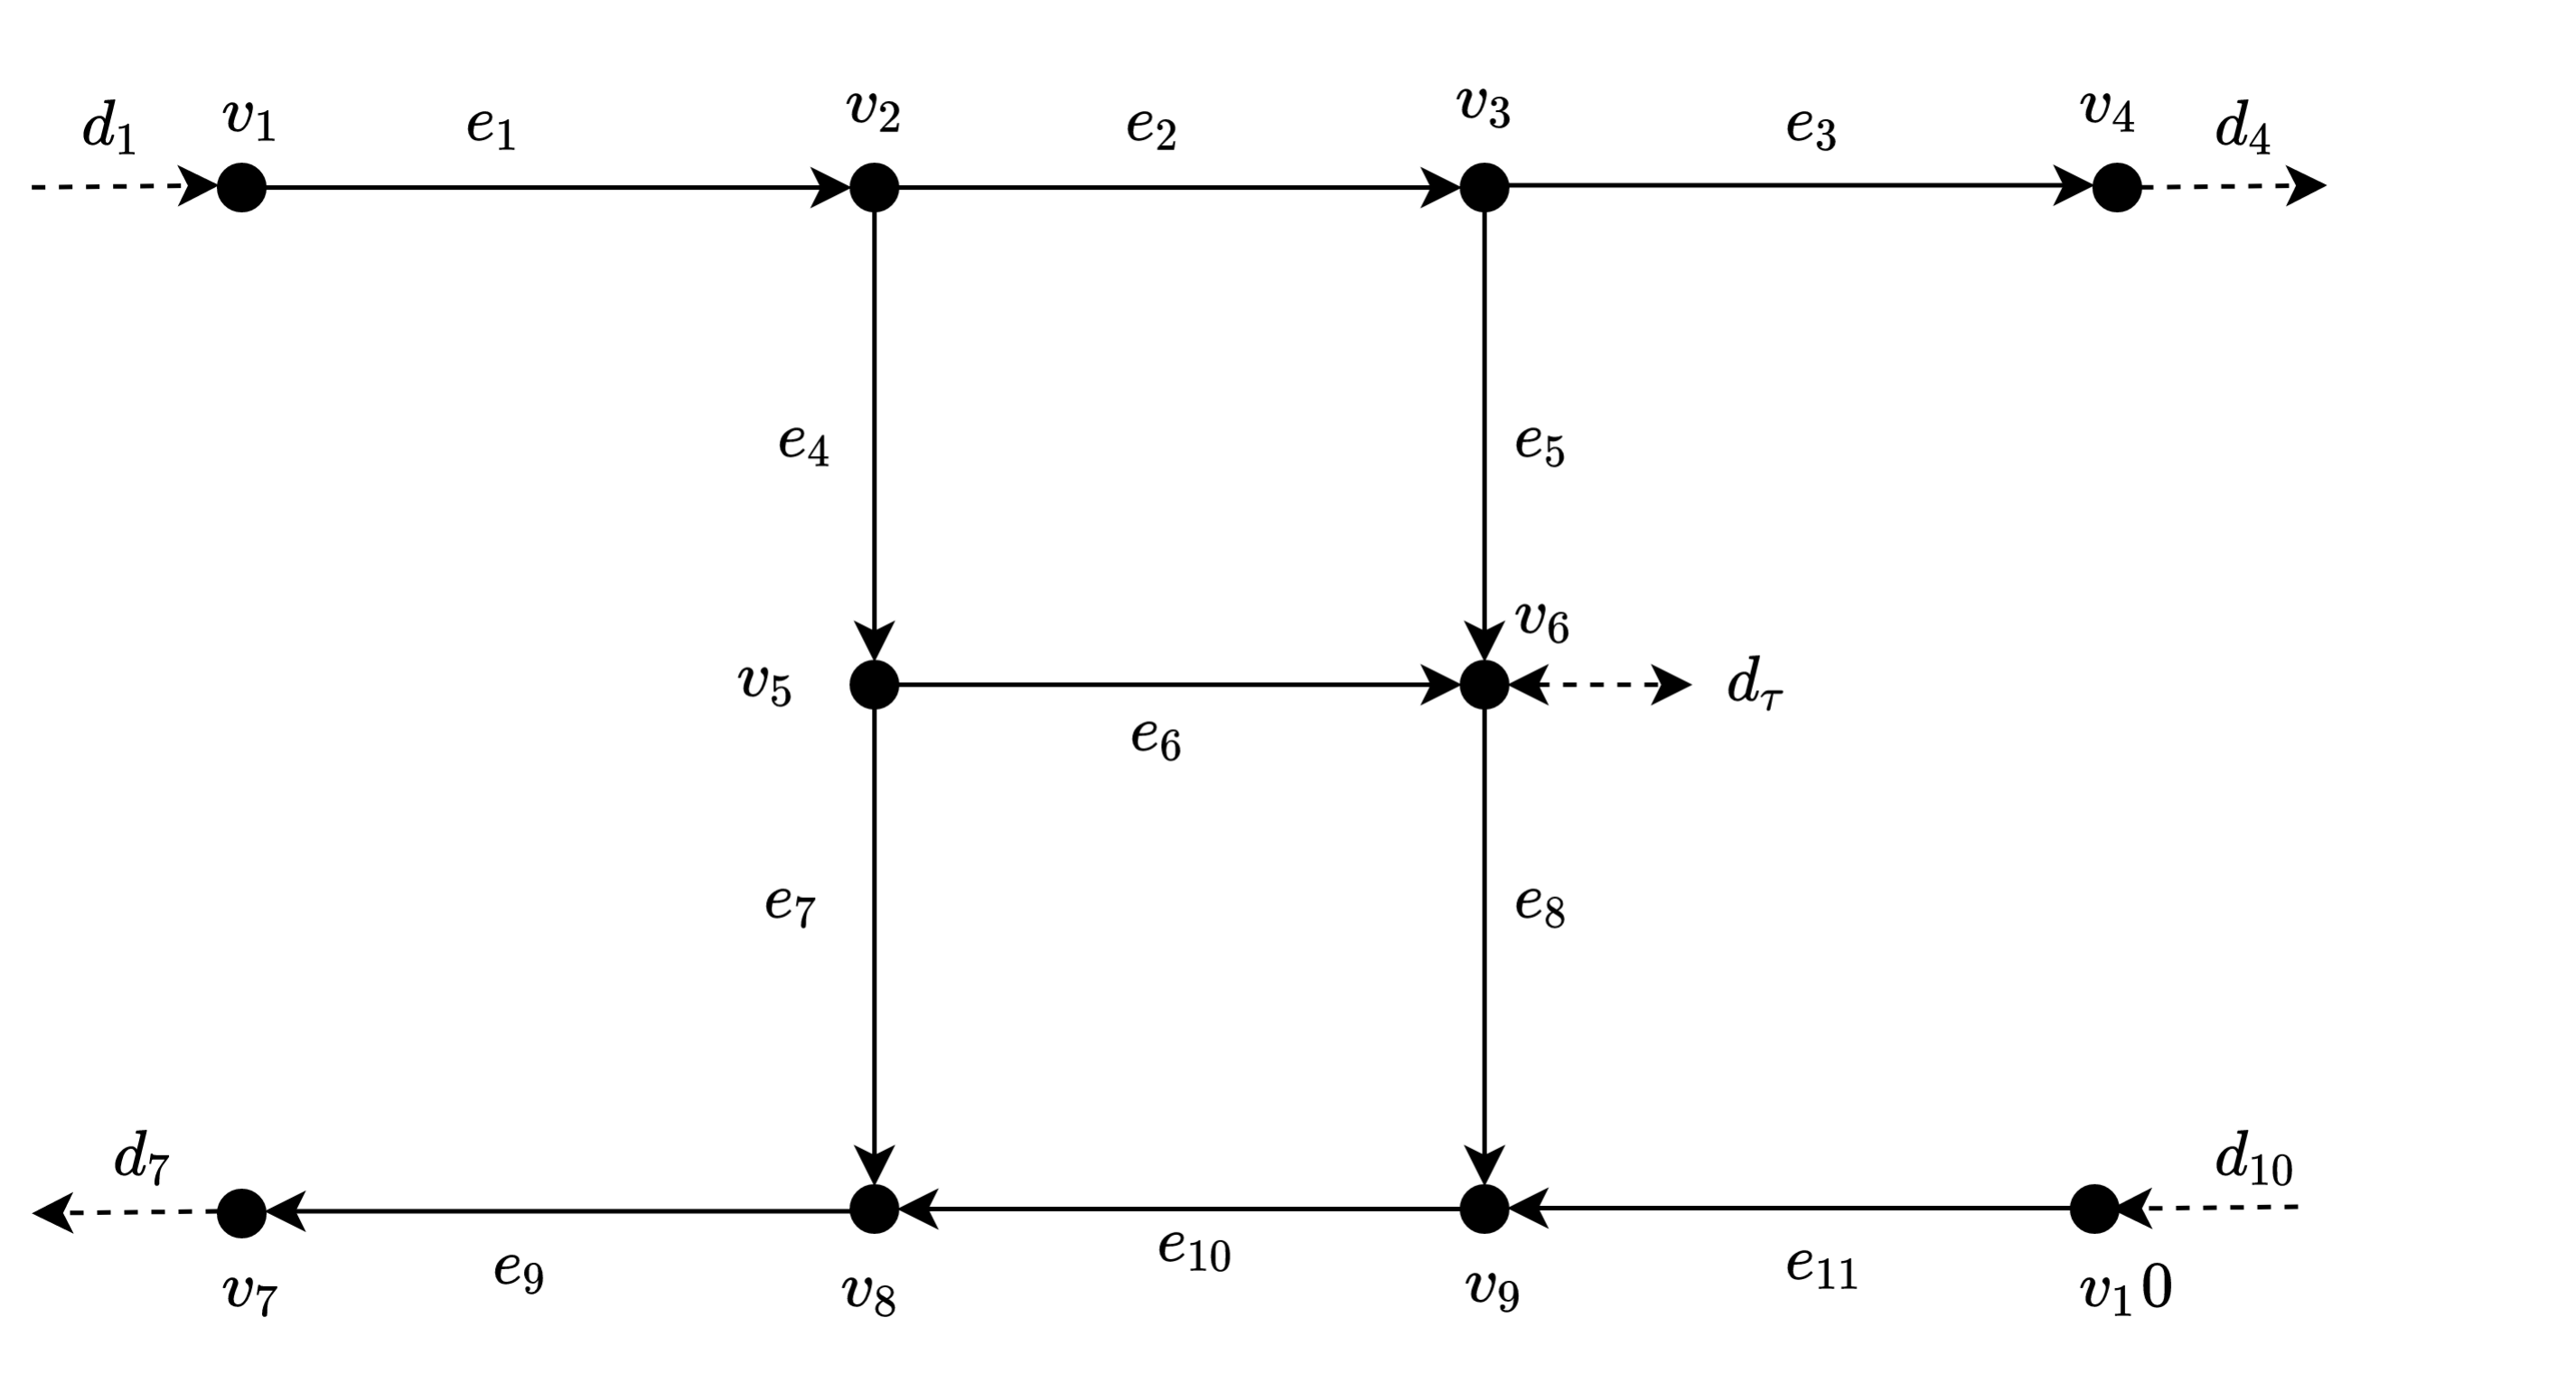
\includegraphics[width=0.7\textwidth]{Pictures/GraphDetailed.png}
	\caption{Detailed graph model of WDN} 
		\label{fig:WDNDetailed}
	\end{figure}
	
	\begin{equation}
		H = \begin{bmatrix}
			1 & 0 & 0   & 0  & 0  & 0  & 0  & 0  & 0  & 0  & 0 \\
			-1 & 1 & 0  & 1  & 0  & 0  & 0  & 0  & 0  & 0  & 0 \\
			0 & -1 & 1  & 0  & 1  & 0  & 0  & 0  & 0  & 0  & 0 \\
			0 & 0  & -1 & 0  & 0  & 0  & 0  & 0  & 0  & 0  & 0 \\
			0 & 0  & 0  & -1 & 0  & 1  & 1  & 0  & 0  & 0  & 0 \\
			0 & 0  & 0  & 0  & -1 & -1 & 0  & 1  & 0  & 0  & 0 \\
			0 & 0  & 0  & 0  & 0  & 0  & 0  & 0  & -1 & 0  & 0 \\
			0 & 0  & 0  & 0  & 0  & 0  & -1 & 0  & 1  & -1 & 0 \\
			0 & 0  & 0  & 0  & 0  & 0  & 0  & -1 & 0  & 1  & -1 \\
			0 & 0  & 0  & 0  & 0  & 0  & 0  & 0  & 0  & 0  & 1 
		\end{bmatrix}
	\end{equation}	
	
\begin{equation*} 
	\begin{split}
		H_{C} &= \{e_{2},e_{6}\}   \\ E_{T} &= \{e_1,e_3,e_4,e_5,e_7, e_8, e9, e10 , e_11\}
	\end{split}
\end{equation*}	
	
	By removing $v_{6}$ from $H$ we get $\bar{H}$ which results in:
	\begin{equation}
		\bar{H} = \begin{bmatrix}
			1 & 0 & 0   & 0  & 0  & 0  & 0  & 0  & 0  & 0  & 0 \\
			-1 & 1 & 0  & 1  & 0  & 0  & 0  & 0  & 0  & 0  & 0 \\
			0 & -1 & 1  & 0  & 1  & 0  & 0  & 0  & 0  & 0  & 0 \\
			0 & 0  & -1 & 0  & 0  & 0  & 0  & 0  & 0  & 0  & 0 \\
			0 & 0  & 0  & -1 & 0  & 1  & 1  & 0  & 0  & 0  & 0 \\
			
			0 & 0  & 0  & 0  & 0  & 0  & 0  & 0  & -1 & 0  & 0 \\
			0 & 0  & 0  & 0  & 0  & 0  & -1 & 0  & 1  & -1 & 0 \\
			0 & 0  & 0  & 0  & 0  & 0  & 0  & -1 & 0  & 1  & -1 \\
			0 & 0  & 0  & 0  & 0  & 0  & 0  & 0  & 0  & 0  & 1 
		\end{bmatrix}
	\end{equation}
	
	
	
	\begin{equation*}
		M_{p} = \begin{bmatrix}
			1 & 0\\
			0 & 0\\
			0 & 0\\
			0 & 0\\
			0 & 0\\
			0 & 0\\
			0 & 0\\
			0 & 0\\
			0 & 0\\
			0 & 1
		\end{bmatrix},
		M_{c} = \begin{bmatrix}
			0 & 0\\
			0 & 0\\
			0 & 0\\
			1 & 0\\
			0 & 0\\
			0 & 0\\
			0 & 1\\
			0 & 0\\
			0 & 0\\
			0 & 0
		\end{bmatrix},
		M_{t} = \begin{bmatrix}
			0\\
			0\\
			0\\
			0\\
			0\\
			1\\
			0\\
			0\\
			0\\
			0
		\end{bmatrix}
	\end{equation*}
	
	
	

